\chapter{Vizualizacija podatkov}

V prejšnjih poglavjih smo obravnavali predvsem modeliranje podatkov in metode, s katerimi iz podatkov gradimo napovedne ali opisne modele. Pri tem smo se vizualizacije že večkrat, morda le bežno, dotaknili, na primer pri predstavitvi modelov (nomogrami), rezultatih zmanjšanja dimenzij (PCA in t-SNE) ter razlagah točkovnih grafov. A o vizualizaciji podatkov še nismo sistematično spregovorili in čas je, da to storimo, saj je vizualizacija ključna pri predstavitvi celotnega procesa in rezultatov tehnik odkrivanja znanja iz podatkov.

Vizualizacija podatkov je samostojno področje, ki raziskuje, kako podatke (in modele) predstaviti tako, da jih lahko zaznamo, razumemo in interpretiramo. Znanost grafične komunikacije podatkov (angl. \emph{visual data communication}) povezuje računalništvo, statistiko, kognitivno psihologijo, oblikovanje in raziskave človeške percepcije. Njeno osnovno vprašanje je presenetljivo preprosto: kako podatke prikazati tako, da bomo v njih čim hitreje in čim bolj pravilno opazili vzorce, razlike, povezave in odstopanja.

Dobro zasnovana vizualizacija temelji na dejstvu, da je človekov vidni sistem izjemno zmogljiv pri zaznavanju struktur, trendov in anomalij.
%
\marginnote{Naš vidni sistem je rezultat evolucijske prilagoditve na hitro zaznavanje struktur, kontrastov, gibanja in anomalij v prostoru. Prav zato lahko grafične predstavitve podatkov pogosto razumemo bistveno hitreje kot numerične tabele.
}
%
Pogosto lahko iz grafa skoraj v trenutku razberemo zakonitosti, ki bi jih iz tabelaričnih podatkov ali statističnih povzetkov težko opazili. Vizualizacija tako ni le sredstvo za prikaz rezultatov, ampak pomembno orodje analize podatkov. 

V podatkovni znanosti vizualizacijo uporabljamo v različnih fazah dela. Najprej kot orodje raziskovalne analize podatkov (angl. \emph{exploratory analysis} in \emph{exploratory visualization}), kjer podatkovni znanstveniki oziroma analitiki z grafičnimi prikazi preverjamo porazdelitve, iščemo osamelce, ocenjujemo povezave med atributi in odkrivamo morebitne napake v podatkih. Vizualizacija je pogosto tudi najhitrejši način za razhroščevanje podatkov, saj so napačno kodirani atributi, manjkajoče vrednosti ali nenavadne meritve na dobrem grafu pogosto takoj opazne. Pomembno vlogo ima tudi pri oblikovanju hipotez, saj nas vizualni vzorci pogosto usmerijo k vprašanjem, ki jih brez grafične predstavitve sploh ne bi zastavili. Druga pomembna vloga vizualizacije je komunikacija rezultatov, kjer je cilj podajanje naših ugotovitev, ki sledijo iz podatkov, drugim, torej ciljnemu občinstvu. Pojasnjevalna vizualizacija (\emph{explanatory visualization}) je namenjena občinstvu ter skuša jasno in učinkovito prenesti sporočilo. Dober raziskovalni graf je lahko neurejen, poln informacij in namenjen hitremu preverjanju idej; dober pojasnjevalni graf pa mora biti jasen, osredotočen in prilagojen ciljnemu občinstvu.

Raziskave na področju vizualizacije so pokazale, da različni grafični elementi niso enako učinkoviti. Človek na primer precej natančneje primerja položaje točk na osi kot pa površine krogov ali intenziteto barv. Zato izbira načina prikaza podatkov ni zgolj estetsko vprašanje, ampak neposredno vpliva na pravilnost interpretacije. Napačno izbrane vizualizacije lahko podatke popačijo, zavedejo opazovalca ali prikrijejo pomembne zakonitosti.

Tu bomo obravnavali osnovna načela vizualizacije podatkov in pregledali najpomembnejše tipe grafičnih prikazov. Zanimalo nas bo, kako različne vrste podatkov učinkovito predstaviti, katere vizualne elemente uporabljamo za prikaz vrednosti in odnosov med podatki ter kako izbrati prikaz, ki ustreza analitični nalogi. Posebej bomo poudarili tudi omejitve posameznih tipov grafičnih predstavitev, omenili nekaj pogostih napak pri načrtovanju vizualizacij in se na kratko posvetili interpretaciji kompleksnih vizualnih predstavitev. Učinkovite vizualizacije, predstavljene na računalnikih, podpirajo interaktivnost, zato bomo omenili tudi področje vizualne analitike (angl. \emph{visual analytics}). Poglavje zaključimo praktično, s pregledom nekaterih programskih pristopov za konstrukcijo vizualizacij.


\subsection{Tipi podatkov}

Pri načrtovanju vizualizacij je najprej potrebno razumeti, kakšne podatke sploh prikazujemo. Različni tipi podatkov zahtevajo različne tipe grafičnih predstavitev, prav tako pa niso vsi vizualni elementi enako učinkoviti pri prikazu posameznih vrst podatkov. Prav zaradi pravilne (ali napačne) uporabe vizualnih dokumentov so lahko nekateri grafi pregledni in informativni, drugi pa zavajajoči ali težko razumljivi.

V podatkovni znanosti običajno ločimo med kategoričnimi, numeričnimi, časovnimi in prostorskimi podatki. Kategorični podatki opisujejo pripadnost skupinam ali razredom. Primeri so spol, vrsta izdelka, država ali oznaka razreda. Pri takih podatkih nas pogosto zanimajo frekvence, deleži ali primerjave med skupinami. Numerični podatki predstavljajo merljive količine, kot so temperatura, dohodek, masa ali starost. Pri njih nas zanimajo porazdelitve, povprečja, korelacije in trendi. Posebna vrsta numeričnih podatkov so časovni podatki, kjer vrednosti opazujemo skozi čas. Takšne podatke pogosto predstavljamo z linijskimi grafi, saj želimo poudariti razvoj ali spremembo skozi čas. Prostorski podatki pa vključujejo geografsko ali drugo prostorsko komponento, zato jih pogosto prikazujemo na zemljevidih ali prostorskih mrežah.

\begin{figure}[t]
\centering
% sem pride slika različnih tipov podatkov
\includegraphics[width=.95\linewidth]{figs/100-viz-data-types.pdf}
\caption{Primeri različnih tipov podatkov: kategorični podatki (stolpčni graf), numerični podatki (histogram), časovni podatki (linijski graf) in prostorski podatki (zemljevid).
\protect\label{fig:data-types}}
\end{figure}

Slika~\ref{fig:data-types} prikazuje tipične primere vizualizacij za različne vrste podatkov. Že iz teh primerov je razvidno, da izbira grafične predstavitve ni naključna. Linijski graf je primeren za prikaz časovnih sprememb, histogram za prikaz porazdelitve numeričnih podatkov, zemljevid pa za prikaz prostorske razporeditve.

Pomembna je tudi dimenzionalnost podatkov. Pri enorazsežnih oziroma univariatnih podatkih (\emph{univariate data}) analiziramo eno samo spremenljivko. Zanima nas na primer porazdelitev starosti ali višine oseb. Pri dvodimenzionalnih oziroma bivariatnih podatkih proučujemo odnos med dvema spremenljivkama, na primer povezavo med višino in telesno maso. Večrazsežni oziroma multivariatni podatki vsebujejo več atributov hkrati in zahtevajo bolj kompleksne vizualizacije.

\begin{figure}[t]
\centering
% sem pride slika univariatnih, bivariatnih, trivariatnih in multivariatnih podatkov
\includegraphics[width=.95\linewidth]{figs/100-viz-dim.pdf}
\caption{Grafični prikazi za različne dimenzionalnosti vizualiziranih podatkov: histogram za univariatne podatke, razsevni diagram za bivariatne podatke, mehurčni diagram za trivariatne podatke in paralelne koordinate za multivariatne podatke.
\protect\label{fig:data-dimensionality}}
\end{figure}

Slika~\ref{fig:data-dimensionality} prikazuje vizualizacije prilagojene različnim dimenzionalnostim podatkov. Histogram omogoča vpogled v porazdelitev ene same spremenljivke, razsevni diagram prikazuje povezavo med dvema spremenljivkama, paralelne koordinate
%
\marginnote{Prikaz s paralelnimi koordinatami hitro postane nepregleden pri večjem številu primerov ali atributov, saj se črte prekrivajo in otežijo zaznavanje vzorcev ter povezav med spremenljivkami, sama vizualizacija in nje interpretacija pa postane močno odvisna od vrstnega reda atributov.}
%
pa omogočajo prikaz več atributov hkrati. Z naraščanjem števila dimenzij postaja interpretacija vizualizacij vse zahtevnejša, zato je pomembno izbrati prikaz, ki omogoča preglednost tudi pri večji kompleksnosti podatkov. 

\section{Vizualni elementi}

Vizualizacije temeljijo na preslikavi podatkov v vizualne elemente oziroma vizualne kanale. Ti določajo, kako bodo podatki predstavljeni opazovalcu. Najpomembnejši vizualni elementi so položaj, dolžina, kot, površina, barva, oblika in velikost.

Položaj je najpomembnejši in hkrati najnatančnejši vizualni element. Človek zelo dobro zaznava razlike v položaju točk na skupni osi, zato so razsevni diagrami, linijski grafi in stolpčni grafi pogosto zelo učinkoviti. Dolžina je prav tako zelo dobro zaznavna in jo uporabljamo predvsem pri stolpčnih grafih. Precej manj natančno zaznavamo kote in površine, zato so tortni diagrami pogosto slabša izbira od stolpčnih grafov. Barva je izredno uporabna za ločevanje skupin, označevanje intenzitete ali poudarjanje pomembnih delov podatkov, vendar človek razlik v intenziteti barv ne zaznava posebej natančno. Oblika in velikost sta predvsem pomožna vizualna elementa za razlikovanje kategorij ali poudarjanje posameznih primerov.

\begin{figure}[t]
\centering
% sem pride shema vizualnih kanalov
\includegraphics[width=.95\linewidth]{figs/100-viz-visual-channels.pdf}
\caption{Najpogostejši vizualni elementi za predstavitev podatkov: položaj, dolžina, kot, površina, barva, oblika in velikost. Vizualni elementi se razlikujejo po natančnosti, s katero človek zaznava kvantitativne razlike.
\protect\label{fig:visual-channels}}
\end{figure}

Na sliki~\ref{fig:visual-channels} so prikazani nekateri pogosti vizualni elementi. Pomembno je razumeti, da različni elementi niso enako učinkoviti. Položaj in dolžina omogočata zelo natančne primerjave med vrednostmi, medtem ko primerjava površin ali kotov pogosto vodi do napačnih ocen (tabela~\ref{tab:vis-elements}). Prav zato so nekateri tipi grafov bolj primerni za analitično delo kot drugi.

\begin{table}[t]
\centering
\caption{Vizualni elementi za predstavitev podatkov in njihove lastnosti.
\protect\label{tab:vis-elements}}
\footnotesize
\begin{tabular}{p{2.0cm}p{3.0cm}p{3.0cm}p{1.7cm}}
\toprule
\textbf{Vizualni element} & \textbf{Tipična uporaba} & \textbf{Primeri} & \textbf{Zaznavna natančnost} \\
\midrule
Položaj & Primerjava vrednosti & Razsevni diagrami & Zelo visoka \\
Dolžina & Primerjava količin & Stolpčni grafi & Visoka \\
Kot & Prikaz deležev & Tortni diagrami & Srednja \\
Velikost & Poudarjanje pomembnosti & Mehurčni diagrami & Srednja \\
Orientacija & Smer ali usmerjenost & Vektorska polja & Srednja \\
Oblika & Razlikovanje kategorij & Označevalci točk & Omejena \\
Tekstura & Razlikovanje področij & Kartografija & Omejena \\
Ukrivljenost & Prikaz trendov ali tokov & Diagrami povezav & Omejena \\
Barva & Skupine ali intenziteta & Toplotni zemljevidi & Nizka \\
Svetlost & Intenziteta ali gostota & Sivinske skale & Nizka \\
Površina & Velikost količine & Mehurčni diagrami & Nizka \\
Volumen & 3D prikazi količin & 3D stolpci & Zelo nizka \\
\bottomrule
\end{tabular}
\end{table}

Pri načrtovanju vizualizacij moramo zato razumeti tako podatke kot tudi način, kako ljudje zaznavamo vizualne elemente. Preden izberemo grafični prikaz, moramo vedeti, kakšne podatke imamo, kakšne odnose želimo prikazati in kako človek zaznava posamezne vizualne elemente. Šele nato lahko izberemo vizualizacijo, ki bo podatke predstavila jasno, učinkovito in brez zavajanja.

\section{Osnovni tipi grafov}

Izbira vizualizacije je seveda odvisna od vprašanja, na katerega želimo odgovoriti s podatki. Različni grafi poudarjajo različne lastnosti podatkov: porazdelitve, trende, povezave, negotovost ali strukturo. Univerzalno najboljši graf ne obstaja, obstajajo pa dobre in slabe vizualizacije. Vsak tip grafa je primeren za določen analitični cilj in lahko zavaja, če ga uporabimo v neprimernem kontekstu, po drugi strani pa ga lahko uporabimo tako, da primerno izpostavi idejo ali vzorec, zaradi katerega smo se odločili podatke grafično prikazati. 

V nadaljevanju predstavimo nekaj osnovnih tipov grafov. Pri vsakem tipu grafa bomo obravnavali:
\begin{itemize}
\item na kakšno vprašanje odgovarja,
\item kakšne so njegove prednosti in omejitve,
\item katere so tipične pogoste napake pri njegovi uporabi ali interpretaciji.
\end{itemize}

\vspace{1em}
\noindent {\bf Histogram.}
Histogram (slika~\ref{fig:histogram}) prikazuje porazdelitev numerične spremenljivke tako, da razdeli območje vrednosti v intervale (koše) in prikaže število primerov v posameznem intervalu. 
%
\begin{marginfigure}
\includegraphics[width=\linewidth]{figs/100-histogram-example.pdf}
\caption{Histogram porazdelitve rezultatov izpita. Graf razkrije asimetrijo in morebitno večvršnost porazdelitve.
\protect\label{fig:histogram}}
\end{marginfigure}
%
Histogrami odgovarjajo na vprašanja:
\begin{itemize}
\item Ali je porazdelitev simetrična ali asimetrična?
\item Ali vsebuje več vrhov?
\item Ali so prisotni osamelci?
\item Ali je porazdelitev približno normalna?
\end{itemize}

Histogrami omogočajo hiter vpogled v obliko porazdelitve podatkov. Primerni so za raziskovalno analizo in hitro razumevanje oblike podatkov. Pri histogramih rezultat močno vpliva izbira širine intervalov. Preširoki intervali skrijejo strukturo, preozki pa poudarijo šum v podatkih.

Pogosta napaka je primerjanje histogramov z različno velikimi intervali ali različnimi velikostmi vzorca brez ustrezne normalizacije. Histogrami tudi niso primerni za podatke z majhnim številom primerov, na primer, kadar imamo le nekaj deset opazovanj, saj lahko oblika porazdelitve tedaj močno zavisi od izbire intervalov in naključnih odstopanj v podatkih.

\vspace{1em}
\noindent {\bf Škatla z brki.}
Škatla z brki (angl. {\em box-and-whisker plot}, slika~\ref{fig:boxplot}) povzema porazdelitev numerične spremenljivke s kvartili in osamelci. Osamelci so podatkovne točke, ki ležijo več kot 1,5 medkvartilnega razmika nad tretjim kvartilom ali pod prvim kvartilom.
%
\begin{marginfigure}
\includegraphics[width=\linewidth]{figs/100-boxplot.pdf}
\caption{Škatlasti diagram z brki prikazuje porazdelitev odzivnih časov treh algoritmov. Črna črta v škatli označuje mediano, robova škatle predstavljata prvi in tretji kvartil, brki segajo do najbolj oddaljenih vrednosti brez osamelcev, krogi pa označujejo osamelce.
\protect\label{fig:boxplot}}
\end{marginfigure}
%
Odgovarja na vprašanja:
\begin{itemize}
\item Kakšna je mediana podatkov?
\item Kako velika je variabilnost?
\item Ali so prisotni osamelci?
\item Kako se porazdelitve razlikujejo med skupinami?
\end{itemize}
%
Škatlasti diagrami omogočajo kompaktno primerjavo več skupin hkrati. Pri tem pa izgubimo podrobnejši vpogled v obliko porazdelitve. Dve zelo različni porazdelitvi lahko ustvarita skoraj enako vizualizacijo. Pogosta napaka je interpretacija osamelcev kot napak merjenja. Osamelci lahko predstavljajo pomembne redke dogodke. Škatle z brki niso primerne za zelo majhne vzorce.

\vspace{1em}
\noindent {\bf Violinski diagram.}
Violinski diagram (angl. {\em violin plot}, slika~\ref{fig:violin}) razširi škatlasti diagram z brki z oceno gostote porazdelitve podatkov. Širina violine predstavlja gostoto podatkov pri posamezni vrednosti: širši deli označujejo območja z več opazovanji. V prikazu so posamezna opazovanja prikazana s točkami, črna črta pa označuje mediano.
%
\begin{marginfigure}
\includegraphics[width=\linewidth]{figs/100-violinplot.pdf}
\caption{Violinski diagram prikazuje porazdelitve čakalnih časov v različnih trgovinah. Širina violine predstavlja gostoto podatkov, točke posamezna opazovanja, črna črta pa mediano.
\protect\label{fig:violin}}
\end{marginfigure}
%
Odgovarja na enaka vprašanja kot škatla z brki, dodatno pa razkrije:
\begin{itemize}
\item večvršnost porazdelitve,
\item asimetrijo,
\item podrobnejšo strukturo podatkov,
\item območja z večjo koncentracijo opazovanj.
\end{itemize}

Violinski diagrami prikažejo tudi gostoto in strukturo porazdelitve. Prikaz je občutljiv na izbiro metode glajenja pri oceni gostote. Navidezni vrhovi ali doline so lahko posledica izbire parametrov glajenja in ne dejanske strukture podatkov. Pogosta napaka je uporaba violinskih diagramov pri zelo majhnih vzorcih, kjer ocena gostote ni zanesljiva.

\vspace{1em}
\noindent {\bf Razsevni diagram.}
Razsevni diagram (angl. {\em scatter plot}, slika~\ref{fig:scatter}) prikazuje odnos med dvema numeričnima spremenljivkama. Vsaka točka predstavlja eno opazovanje, njen položaj pa določata vrednosti obeh spremenljivk. Diagram omogoča vizualno prepoznavanje povezav, trendov, gruč in osamelcev.
%
\begin{marginfigure}
\includegraphics[width=\linewidth]{figs/100-scatterplot.pdf}
\caption{Razsevni diagram prikazuje povezavo med časom učenja in rezultatom izpita. Vsaka točka predstavlja posameznega študenta, črta pa linearni trend med obema spremenljivkama. Opazen je tudi osamelec, ki odstopa od splošnega vzorca podatkov.}
\protect\label{fig:scatter}
\end{marginfigure}
%
Odgovarja na vprašanja:
\begin{itemize}
\item Ali sta spremenljivki povezani?
\item Ali je povezava linearna ali nelinearna?
\item Ali obstajajo gruče ali podskupine?
\item Ali so prisotni osamelci?
\item Kako močna je povezanost med spremenljivkama?
\end{itemize}

Razsevni diagram neposredno pokaže odnos med spremenljivkama. Pogosto sodijo med najpomembnejša orodja raziskovalne analize podatkov, saj omogočajo hitro prepoznavanje trendov, vzorcev in nepravilnosti. Njihova glavna omejitev je prekrivanje točk pri velikih podatkovnih množicah, kjer gosta območja postanejo težko berljiva. Takrat si pogosto pomagamo s prosojnostjo točk, vzorčenjem ali alternativnimi prikazi gostote.

Pogosta napaka pri interpretaciji razsevnih diagramov je sklepanje o vzročnosti na podlagi korelacije. Diagram prikazuje povezanost med spremenljivkama, ne pa nujno vzročnega odnosa.

\vspace{1em}
\noindent {\bf Črtni diagram.}
Črtni diagram (angl. {\em line chart}, slika~\ref{fig:linechart}) prikazuje spremembe vrednosti vzdolž urejene osi, najpogosteje skozi čas. Posamezne meritve so predstavljene s točkami, ki so povezane s črto, kar omogoča vizualno spremljanje trendov, nihanj in sprememb skozi čas.
%
\begin{marginfigure}
\includegraphics[width=\linewidth]{figs/100-linechart.pdf}
\caption{Črtni diagram prikazuje obisk spletne strani skozi čas. Črta povezuje zaporedne meritve in omogoča prepoznavanje trendov ter nenadnih sprememb. Označena sta tudi dva posebna dogodka oziroma vpliv akcij.
\protect\label{fig:linechart}}
\end{marginfigure}
%
Odgovarja na vprašanja:
\begin{itemize}
\item Kako se količina spreminja skozi čas?
\item Ali obstajajo trendi ali sezonski vzorci?
\item Ali so prisotne nenadne spremembe?
\item Kako hitro ali pogosto se vrednosti spreminjajo?
\end{itemize}

Črtni diagrami so posebej primerni za prikaz časovnih trendov in sprememb. Posebej primerni so za prikaz časovnih vrst, kjer želimo poudariti razvoj podatkov skozi čas.

Njihova slabost je implicitna predpostavka zveznosti med zaporednimi točkami, ki ni vedno smiselna. Pri velikem številu serij ali zelo gostih meritvah lahko graf hitro postane nepregleden. Pogosta napaka pri uporabi tega grafa je povezovanje kategoričnih podatkov s črto, kar ustvarja vtis neobstoječe zveznosti. Težava je tudi prikaz preveč podatkovnih serij hkrati, saj to oteži primerjavo in interpretacijo.


\vspace{1em}
\noindent {\bf Stolpčni diagram.}
Stolpčni diagram (angl. {\em bar chart}, slika~\ref{fig:barchart}) primerja količine med kategorijami. Dolžina oziroma višina stolpcev predstavlja vrednost posamezne kategorije, kar omogoča hitro vizualno primerjavo med skupinami.
%
\begin{marginfigure}
\includegraphics[width=\linewidth]{figs/100-barchart.pdf}
\caption{Stolpčni diagram primerja prodajo med kategorijami izdelkov. Višina stolpcev predstavlja prodajo posamezne kategorije.
\protect\label{fig:barchart}}
\end{marginfigure}
%
Odgovarja na vprašanja:
\begin{itemize}
\item Katera kategorija ima največjo ali najmanjšo vrednost?
\item Kako velike so razlike med skupinami?
\item Kakšen je vrstni red kategorij?
\item Katere kategorije izstopajo?
\end{itemize}

Stolpčne diagrame običajno hitro in intuitivno razumemo. Posebej primerni so za predstavitev agregiranih podatkov in primerjanje kategorij širšemu občinstvu.

Njihova omejitev je, da prikazujejo predvsem povzetke podatkov in skrijejo variabilnost znotraj skupin. Pri večjem številu kategorij lahko diagram hitro postane nepregleden. Pogosta napaka je rezanje navpične osi, saj uporabniki primerjajo dolžine stolpcev. Že majhna sprememba začetka osi lahko močno pretirava ali zmanjša zaznane razlike med kategorijami.


\vspace{1em}
\noindent {\bf Toplotna karta.}
Toplotna karta (angl. {\em heatmap}, slika~\ref{fig:heatmap}) prikazuje vrednosti matrike s pomočjo barvne lestvice. Posamezne celice predstavljajo vrednosti med pari spremenljivk, pri čemer barva označuje velikost ali intenzivnost vrednosti. Toplotne karte omogočajo hitro prepoznavanje vzorcev, povezanosti, gruč in območij z izrazitimi vrednostmi.
%
\begin{marginfigure}
\includegraphics[width=\linewidth]{figs/100-heatmap.pdf}
\caption{Toplotna karta prikazuje korelacijsko matriko med številom ur učenja, prisotnostjo na vajah, številom oddanih nalog, kakovostjo spanja in rezultatom izpita. Vsaka celica predstavlja korelacijo med parom spremenljivk: temno modra označuje močno pozitivno korelacijo, temno rdeča močno negativno korelacijo, svetlejši odtenki pa šibkejšo povezanost. Diagonala vsebuje popolne korelacije spremenljivk s samimi seboj.
\protect\label{fig:heatmap}}
\end{marginfigure}
%
Odgovarja na vprašanja:
\begin{itemize}
\item Katere spremenljivke so močno povezane?
\item Ali obstajajo vzorci ali gruče?
\item Kje so skoncentrirane visoke ali nizke vrednosti?
\item Katere spremenljivke imajo podobno vedenje?
\end{itemize}

Toplotne karte omogočajo hkraten pregled velikega števila vrednosti in povezav med njimi. Posebej uporabne so pri analizi korelacijskih matrik, časovnih vzorcev in drugih strukturiranih podatkov.

Njihova slabost je odvisnost od izbire barvne lestvice in razvrstitve podatkov. Slabo izbrane barve lahko popačijo interpretacijo razlik med vrednostmi ali poudarijo navidezne vzorce. Pri podatkih z naravno sredinsko vrednostjo, kot so korelacije, je smiselna uporaba divergentnih barvnih lestvic z nevtralno sredinsko barvo, na primer modro--belo--rdeče lestvice.

Pogosta napaka je uporaba mavričnih barvnih lestvic, ki ustvarijo umetne kontraste in otežijo interpretacijo. Priporočljive so perceptualno enakomerne barvne lestvice, kjer spremembe v barvi ustrezajo spremembam v podatkih. Za sekvenčne podatke so pogosto primerne lestvice, kot je {\em viridis}, za korelacijske matrike pa divergentne lestvice, kot sta {\em coolwarm} ali {\em RdBu}. Pomembna je tudi zmerna nasičenost barv in dobra čitljivost pri sivinskem prikazu.



\vspace{1em}
\noindent {\bf Matrika razsevnih diagramov.}
Matrika razsevnih diagramov (angl. {\em scatterplot matrix} ali {\em pair plot}, slika~\ref{fig:pairplot}) prikazuje vse parne odnose med več numeričnimi spremenljivkami hkrati. Vsaka celica matrike vsebuje razsevni diagram za izbrani par spremenljivk, diagonala pa pogosto prikazuje porazdelitve posameznih spremenljivk.
%
\begin{marginfigure}
\includegraphics[width=\linewidth]{figs/100-pairplot.pdf}
\caption{Matrika razsevnih diagramov prikazuje parne odnose med številom ur učenja, prisotnostjo na vajah, kakovostjo spanja in rezultatom izpita. Vsaka celica vsebuje razsevni diagram za določen par spremenljivk, diagonala pa prikazuje porazdelitve posameznih spremenljivk. Vidna je pozitivna povezava med časom učenja in rezultatom izpita ter šibkejša povezanost drugih dejavnikov.
\protect\label{fig:pairplot}}
\end{marginfigure}
%
Odgovarja na vprašanja:
\begin{itemize}
\item Katere spremenljivke so povezane?
\item Ali obstajajo gruče ali ločeni razredi?
\item Katere spremenljivke so redundantne?
\item Ali so povezave linearne ali nelinearne?
\item Ali so prisotni osamelci ali nenavadni vzorci?
\end{itemize}

Matrike razsevnih diagramov omogočajo hiter pregled odnosov med več spremenljivkami. Omogočajo istočasno prepoznavanje korelacij, gruč, osamelcev in morebitnih nelinearnih povezav.

Njihova glavna slabost je slaba skalabilnost. Število grafov raste kvadratno s številom spremenljivk, zato matrike hitro postanejo nepregledne. Pri velikem številu primerov se pojavi tudi prekrivanje točk, kar oteži interpretacijo.

Pogosta napaka je uporaba matrik razsevnih diagramov pri zelo velikem številu spremenljivk ali opazovanj, kjer vizualizacija izgubi preglednost in informativnost.


%%%%

\section{Vizualizacija pri raziskovalni analizi podatkov}

Vizualizacija ima pomembno vlogo pri raziskovalni analizi podatkov (angl. \emph{exploratory data analysis}, EDA). Preden zgradimo modele ali izvedemo zahtevnejše analize, moramo podatke najprej razumeti. Vizualizacija nam omogoča hiter vpogled v strukturo podatkov, kakovost meritev, povezave med atributi in morebitne nenavadne vzorce. Pogosto lahko že preprost graf razkrije zakonitosti, ki jih iz tabelaričnih podatkov ali numeričnih povzetkov težko opazimo. Pri tem nas na primer zanimajo naslednja vprašanja:
%
\begin{itemize}

\item {\bf Kakšna je porazdelitev atributov?}
Za pregled porazdelitev numeričnih atributov uporabljamo predvsem histograme, gostotne diagrame in violinske diagrame. Takšni prikazi nam omogočajo oceno razpršenosti podatkov, večvršnosti porazdelitve ter prisotnosti dolgih repov. Pri kategoričnih podatkih pogosto uporabimo stolpčne diagrame.

\item {\bf Ali so podatki simetrični ali asimetrični?}
Asimetrijo porazdelitve lahko hitro opazimo na histogramih ali gostotnih diagramih. Močno desno asimetrične porazdelitve so pogoste pri finančnih podatkih, številu ogledov spletnih vsebin ali velikosti datotek.

\item {\bf Ali so prisotni osamelci oziroma anomalije?}
Osamelce pogosto odkrivamo s škatlami z brki, razsevnimi diagrami ali časovnimi prikazi. Nenavadne točke lahko predstavljajo napake meritev ali pomembne redke dogodke, kot so goljufive transakcije ali okvare sistemov.

%
\begin{marginfigure}
\includegraphics[width=\linewidth]{figs/100-eda-skewness.pdf}
\caption{Porazdelitev zneskov spletnih naročil je izrazito desno asimetrična: večina naročil ima nizke zneske, nekaj zelo velikih naročil pa tvori dolgi desni rep porazdelitve. Zaradi teh ekstremnih vrednosti je povprečje večje od mediane. Spodaj je prikazana ista porazdelitev po logaritemski transformaciji, ki zmanjša vpliv velikih vrednosti in porazdelitev naredi bolj simetrično ter primernejšo za nadaljnjo analizo in modeliranje.
\protect\label{fig:eda-skewness}}
\end{marginfigure}
%

\item {\bf Ali v podatkih manjkajo vrednosti?}
Manjkajoče vrednosti lahko prikažemo s posebnimi matrikami prisotnosti podatkov ali s toplotnimi kartami. Takšni prikazi pogosto razkrijejo sistemske težave pri zajemu podatkov ali manjkajoče meritve v določenih časovnih obdobjih.

\item {\bf Katere spremenljivke so med seboj povezane?}
Povezave med numeričnimi atributi najpogosteje raziskujemo z razsevnimi diagrami, matrikami razsevnih diagramov in korelacijskimi toplotnimi kartami. Takšni prikazi lahko razkrijejo linearne ali nelinearne povezave ter redundantne atribute.

\item {\bf Ali obstajajo gruče ali podskupine primerov?}
Gruče podobnih primerov lahko pogosto opazimo na razsevnih diagramih ali projekcijah večdimenzionalnih podatkov v ravnino. Takšni prikazi so pomembni pri segmentaciji uporabnikov, analizi dokumentov in bioinformatiki.

\item {\bf Ali podatki vsebujejo trende ali sezonske vzorce?}
Pri časovnih podatkih uporabljamo predvsem črtne diagrame in časovne toplotne karte. Ti omogočajo zaznavanje dolgoročnih trendov, sezonskih vzorcev, periodičnosti in nenadnih sprememb v podatkih.

\end{itemize}

Raziskovalna analiza podatkov ni le uvodni korak projekta, ampak spremlja skoraj celoten proces podatkovnega rudarjenja. Vizualizacijo uporabljamo pri preverjanju kakovosti podatkov, izbiri atributov, razumevanju modelov in interpretaciji rezultatov. Prav zato je vizualizacija eno ključnih orodij sodobne podatkovne znanosti.


%%%%%%%%%%

\section{Nekaj primerov kompleksnih vizualizacij}

V prejšnjih razdelkih smo obravnavali predvsem osnovne tipe grafičnih prikazov, ki jih pogosto uporabljamo pri raziskovalni analizi podatkov in predstavitvi rezultatov. Mnogi resnični podatkovni problemi pa vključujejo bolj kompleksne strukture: hierarhije, omrežja, prostorske tokove ali zelo goste časovne podatke. Pri takih podatkih osnovni grafi pogosto niso več dovolj učinkoviti, zato uporabljamo naprednejše vizualizacijske pristope, ki skušajo v omejenem prostoru prikazati več informacij hkrati.

Kompleksne vizualizacije praviloma niso namenjene zgolj estetskemu učinku. Večina jih nastane kot odgovor na konkreten problem predstavitve podatkov: kako prikazati veliko število časovnih vrst, kako predstaviti hierarhične odnose med objekti, kako razumljivo prikazati omrežje povezav ali kako hkrati prikazati geografski položaj, smer gibanja in količino podatkov. Takšne vizualizacije pogosto zahtevajo nekoliko več časa za razumevanje, vendar lahko po začetnem učenju omogočajo bistveno učinkovitejšo analizo kompleksnih podatkovnih struktur.

\vspace{1em}
\noindent {\bf Horizontni graf.}
Horizontni graf (angl. {\em horizon graph}, slika~\ref{fig:horizon}) je poseben način prikaza časovnih vrst, namenjen predvsem povečanju gostote prikazanih podatkov. Klasični črtni ali površinski graf pri večjem številu časovnih vrst hitro postane nepregleden, saj posamezna serija potrebuje precej navpičnega prostora. Horizontni graf skuša ta problem rešiti tako, da podatke razdeli v več pasov in jih nato zloži enega čez drugega. Osnovna ideja je, da negativne vrednosti zrcalimo nad osnovno os, nato pa višinske pasove zložimo enega čez drugega. S tem močno zmanjšamo potrebno višino grafa, pri čemer ohranimo časovno ločljivost podatkov. Takšni prikazi so posebej uporabni pri nadzornih ploščah in sistemih za spremljanje velikega števila časovnih signalov.
%
\begin{figure}[t]
\centering
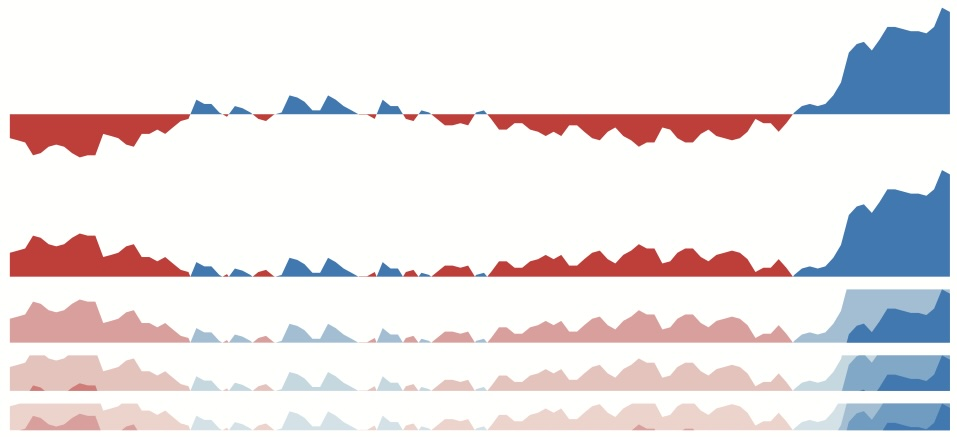
\includegraphics[width=.95\linewidth]{figs/100-horizon-graph.jpg}
\caption{Horizontni graf prikazuje časovno vrsto brezposelnosti skozi čas. Pozitivne in negativne vrednosti so prikazane z različnimi barvami, vrednosti pa so razdeljene v več pasov, ki se prekrivajo. Slika prikazuje tudi postopno transformacijo vizualizacije: od običajnega površinskega grafa, prek zrcaljenja negativnih vrednosti nad osnovno os, do razdelitve podatkov v več nivojev, ki so nato zloženi drug čez drugega. S tem se bistveno poveča gostota prikazanih podatkov, saj lahko enako časovno ločljivost prikažemo na precej manjši površini. Povzeto po Heer in sod. (2010).
\protect\label{fig:horizon}}
\end{figure}
%
Prednost horizontnih grafov je izjemna prostorska učinkovitost. V istem prostoru lahko prikažemo bistveno več podatkov kot s klasičnimi črtnimi diagrami. Slabost pa je nekoliko težje začetno razumevanje prikaza, saj mora opazovalec razumeti zlaganje pasov in pomen barvnih nivojev. Horizontni grafi zato niso najprimernejši za širše občinstvo, zelo uporabni pa so pri analitičnem delu strokovnjakov.

\vspace{1em}
\noindent {\bf Tokovni zemljevid.}
Tokovni zemljevid (angl. {\em flow map}) prikazuje gibanje količin skozi prostor. Takšne vizualizacije pogosto uporabljamo za prikaz migracij, trgovinskih tokov, transporta, širjenja bolezni ali zgodovinskih premikov vojska. Slika~\ref{fig:flow-map} prikazuje znameniti Minardov prikaz Napoleonovega pohoda na Moskvo. Vizualizacija velja za eno najboljših predstavitev podatkov vseh časov, saj v enem samem grafu združuje več različnih dimenzij podatkov. Debelina toka predstavlja velikost vojske, smer toka prikazuje gibanje, položaj predstavlja geografijo, dodatni graf pod zemljevidom pa prikazuje temperaturo med umikom vojske.
%
\begin{figure}[b]
\centering
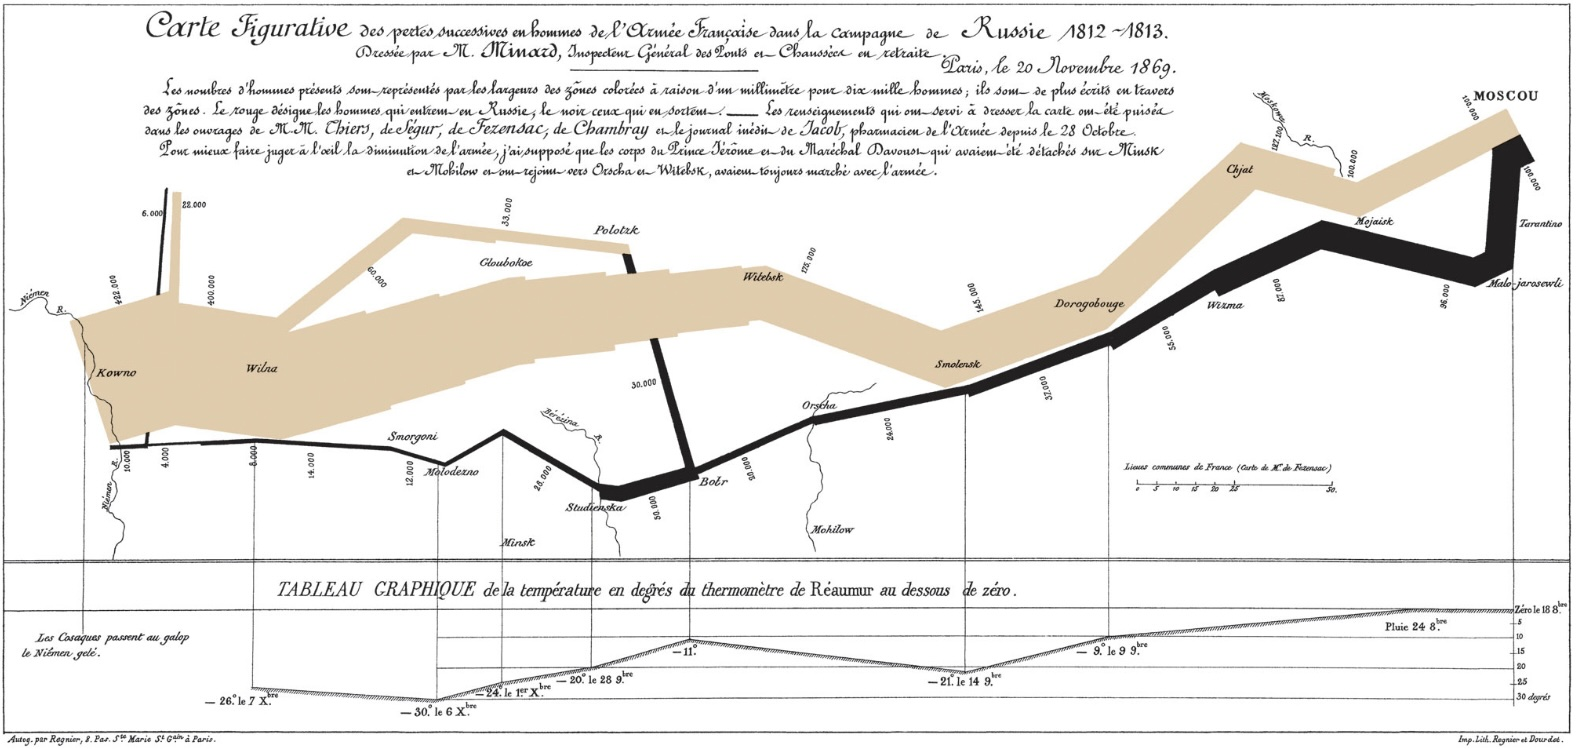
\includegraphics[width=.95\linewidth]{figs/100-flow-map.jpg}
\caption{Tokovni zemljevid Napoleonovega pohoda na Moskvo prikazuje gibanje vojske skozi prostor in čas. Debelina toka predstavlja velikost vojske, položaj označuje geografsko lokacijo, spodnji graf pa prikazuje temperaturo med umikom. Vizualizacija velja za eno najbolj znanih predstavitev večdimenzionalnih podatkov, ki jo je leta 1869 objavil francoski inženir Charles Joseph Minard v delu \emph{Carte figurative des pertes successives en hommes de l'Armée Française dans la campagne de Russie 1812--1813}.
\protect\label{fig:flow-map}}
\end{figure}
%
Tokovni zemljevidi so zanimivi predvsem zato, ker hkrati združujejo prostorske, časovne in količinske informacije. Dobro zasnovan tokovni zemljevid omogoča zelo intuitivno razumevanje kompleksnih procesov gibanja skozi prostor. Njihova slabost pa je možnost velike vizualne nepreglednosti pri večjem številu tokov, saj se poti hitro prekrivajo. Zato pogosto uporabljamo poenostavljanje poti, prosojnost ali interaktivno filtriranje.


\vspace{1em}
\noindent {\bf Drevesni zemljevid.}
Drevesni zemljevid (angl. {\em treemap}) je vizualizacija hierarhičnih podatkov, kjer so elementi predstavljeni z vgnezdenimi pravokotniki. Površina posameznega pravokotnika običajno predstavlja velikost ali pomembnost elementa, hierarhija pa je prikazana z vgnezdenostjo območij.
%
\begin{figure}[t]
\centering
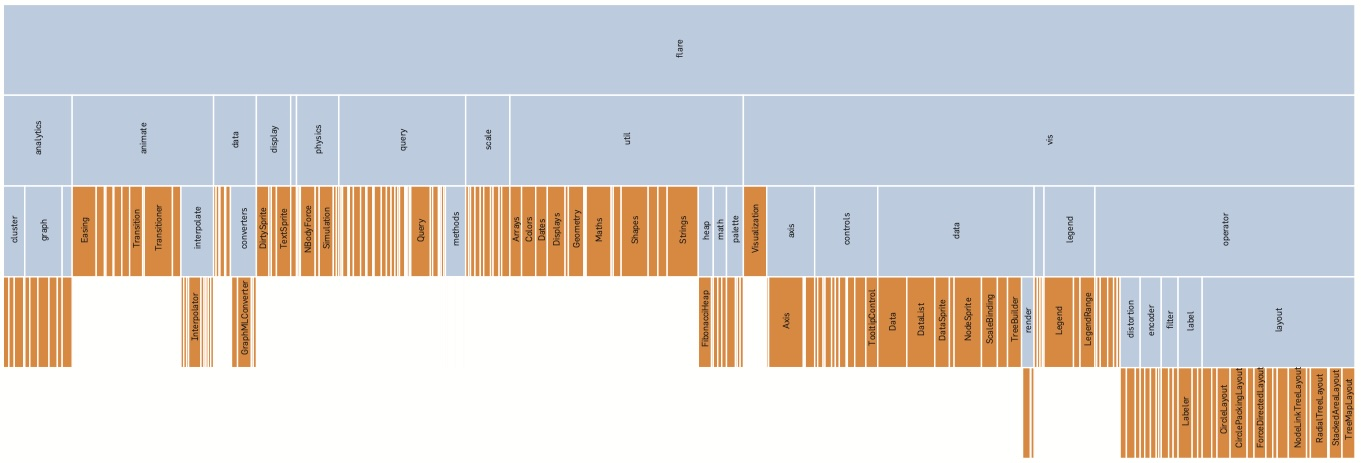
\includegraphics[width=.95\linewidth]{figs/100-treemap.jpg}
\caption{Drevesni zemljevid prikazuje hierarhijo programskih paketov. Posamezni pravokotniki predstavljajo razrede oziroma module, njihova površina pa velikost ali pomembnost posameznega elementa. Povzeto po Heer, Bostock in Ogievetsky, Figure~4f.
\protect\label{fig:treemap}}
\end{figure}
%
Na sliki~\ref{fig:treemap} je prikazan drevesni zemljevid hierarhije programskih paketov. Večji pravokotniki predstavljajo večje oziroma pomembnejše dele sistema. Ker drevesni zemljevid učinkovito izkorišča prostor, lahko na relativno majhni površini prikažemo zelo velike hierarhične strukture. 

Drevesne vizualizacije pogosto uporabljamo za prikaz uporabe diskovnega prostora, strukture finančnih trgov, organizacije datotek ali hierarhičnih klasifikacij. Ti prikazi so posebej uporabni, kadar želimo hitro oceniti relativne velikosti posameznih delov sistema. Njihova prednost je zelo učinkovita izraba prostora in dobra podpora primerjanju velikosti, slabost pa je nekoliko težje sledenje globlji hierarhični strukturi, saj pri zelo velikem številu nivojev vgnezdenost postane nepregledna. Prav tako primerjanje zelo podolgovatih pravokotnikov ni vedno intuitivno.

\vspace{1em}
\noindent {\bf Sončni izsek.}
Sončni izsek (angl. {\em sunburst diagram}) je radialna različica prostorsko zapolnjujoče predstavitve hierarhij. Hierarhija je prikazana s koncentričnimi krožnimi pasovi, kjer notranji krogi predstavljajo višje nivoje hierarhije, zunanji pa nižje nivoje. Na sliki~\ref{fig:sunburst} je prikazan sončni izsek iste hierarhične strukture kot pri drevesnem zemljevidu. V primerjavi z drevesnim zemljevidom sončni izsek pogosto bolj jasno poudari globino hierarhije, saj se nivoji naravno širijo navzven iz središča.

Vizualizacije tega tipa so lahko estetsko zelo privlačne in pogosto uporabljene v interaktivnih sistemih za raziskovanje podatkov. Posebej primerne so za prikaz hierarhičnih struktur, kjer nas zanima predvsem organizacija podatkov in odnosi med nivoji hierarhije. Njihova slabost je nekoliko slabša natančnost pri primerjanju površin in kotov, posebej pri zunanjih segmentih diagrama. Pri zelo globokih hierarhijah postanejo zunanji deli hitro preozki za učinkovito prikazovanje oznak.
%
\begin{marginfigure}
\centering
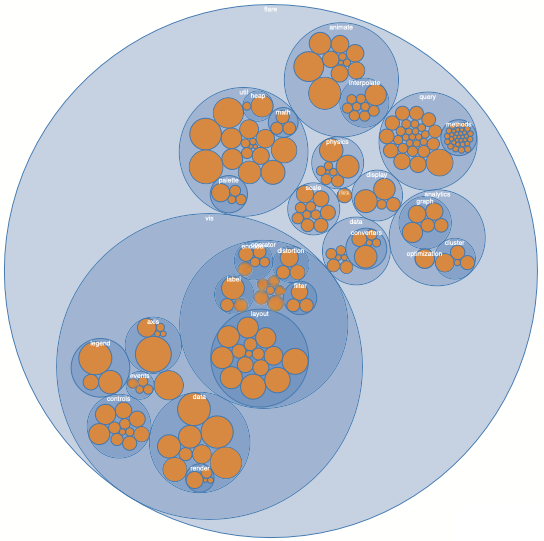
\includegraphics[width=1.0\linewidth]{figs/100-sunburst.png}
\caption{Sončni izsek prikazuje hierarhijo programskih paketov v radialni obliki. Notranji krogi predstavljajo višje nivoje hierarhije, zunanji pa podrobnejše podstrukture. Povzeto po Heer, Bostock in Ogievetsky, Figure~4e.
\protect\label{fig:sunburst}}
\end{marginfigure}
%

\vspace{1em}
\noindent {\bf Vizualizacija omrežij s silami.}
Veliko podatkovnih struktur lahko predstavimo kot omrežje povezav med objekti. Primeri vključujejo socialna omrežja, povezave med spletnimi stranmi, citatne mreže znanstvenih člankov ali biološke interakcije med proteini. Eden najpogostejših pristopov za prikaz takšnih podatkov so razporeditve na osnovi sil (angl. {\em force-directed layouts}).
%
\begin{figure}[t]
\centering
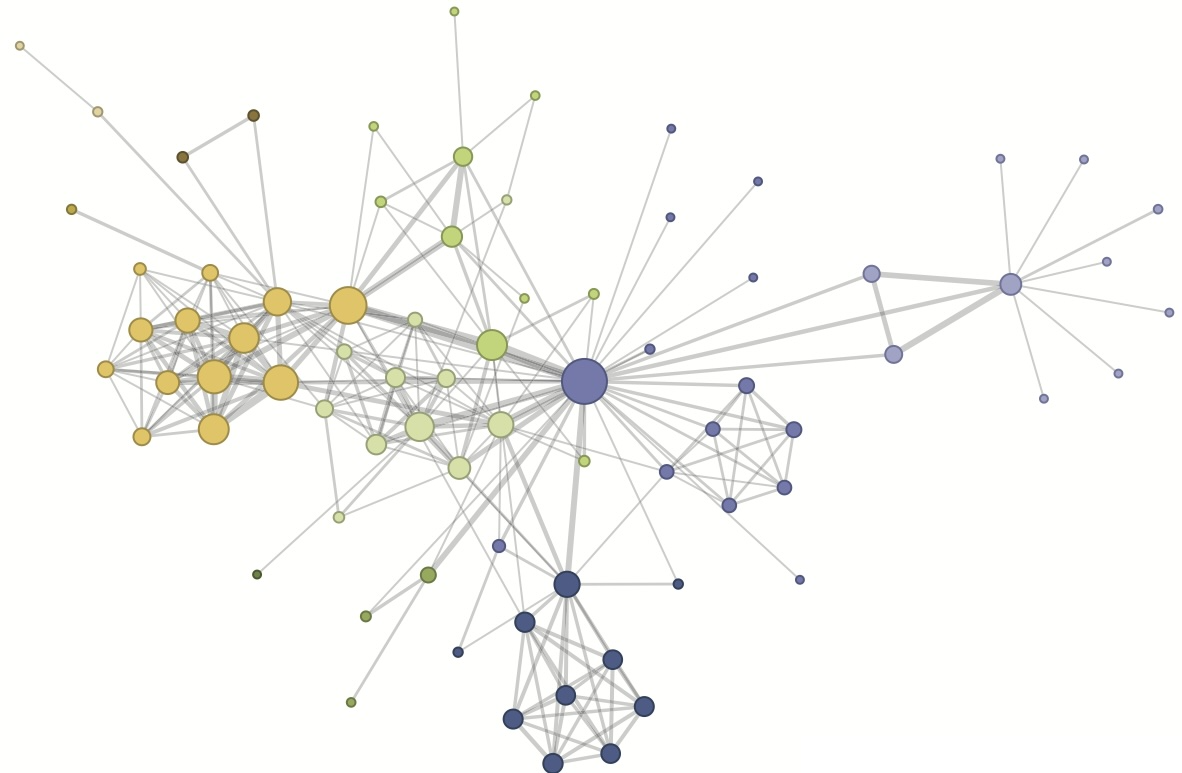
\includegraphics[width=.9\linewidth]{figs/100-force-layout.png}
\caption{Vizualizacija omrežja z razporeditvijo na osnovi sil. Vozlišča predstavljajo literarne like, povezave pa njihove skupne pojavitve v poglavjih romana. Položaj vozlišč je določen s simulacijo privlačnih in odbojnih sil. Povzeto po Heer, Bostock in Ogievetsky, Figure~5a.
\protect\label{fig:force-layout}}
\end{figure}
%
Na sliki~\ref{fig:force-layout} je prikazan primer omrežja likov iz romana \emph{Les Misérables}. Vozlišča predstavljajo posamezne like, povezave pa njihovo skupno pojavljanje v besedilu. Razporeditev vozlišč nastane s simulacijo fizikalnega sistema: povezani elementi se privlačijo, nepovezani pa odbijajo. Posledica je organska razporeditev, kjer se močno povezane skupine naravno združijo v gruče.  Vizualizacije tovrstnih grafov lahko omogočajo hitro prepoznavanje skupin, osrednjih vozlišč in mostov med različnimi deli omrežja. So med najpomembnejšimi pristopi pri analizi socialnih omrežij in kompleksnih grafov. Njihova glavna težava je uporaba na velikih podatkih. Pri zelo velikih omrežjih postanejo povezave nepregledne in vizualizacija se spremeni v tako imenovani klobčič povezav (angl. {\em hairball}), kjer posameznih struktur ni več mogoče razločiti. Zato pri večjih omrežjih pogosto uporabljamo filtriranje, združevanje vozlišč ali alternativne matrične predstavitve omrežij.

Pri sodobni podatkovni analizi pogosto uporabljamo tudi kompleksnejše vizualizacijske pristope. Njihov cilj ni zgolj estetska predstavitev podatkov, ampak učinkovito razkrivanje struktur, odnosov in vzorcev, ki jih z osnovnimi grafi težko opazimo. Pri njihovi uporabi pa moramo biti posebej pozorni na ravnotežje med informativnostjo in razumljivostjo. Če v isti prikaz vključimo preveč informacij, lahko vizualizacija hitro postane nepregledna. Zato je pri načrtovanju kompleksnih vizualizacij še posebej pomembno razumevanje podatkov, naloge analize in omejitev človekovega zaznavanja.



%%%%%%%%%%%%%%%

\section{Načela učinkovitega vizualnega oblikovanja}

Dobra vizualizacija mora opazovalcu omogočiti hitro, pravilno in čim manj naporno razumevanje podatkov. Zato pri načrtovanju grafov ni pomembna le izbira tipa vizualizacije, ampak tudi način uporabe barv, organizacija informacij, poudarjanje ključnih podatkov in odstranjevanje nepomembnih elementov.
%
\marginnote{Nekateri primeri v tem razdelku so povzeti po članku Jonathana Schwabisha \emph{The Practice of Visual Data Communication: What Works} iz revije \emph{Psychological Science in the Public Interest} (2021), ki na praktičnih primerih prikazuje vpliv oblikovnih odločitev na učinkovitost vizualizacij.}
%
Raziskave na področju vizualne percepcije kažejo, da lahko že majhne oblikovne odločitve močno vplivajo na interpretacijo podatkov. Vizualizacija mora zato podpirati človekove zaznavne sposobnosti in zmanjševati kognitivno obremenitev opazovalca. Cilj ni ustvarjanje vizualno spektakularnih grafov, ampak jasna in učinkovita komunikacija podatkov.

\vspace{1em}
\noindent {\bf Preprostost in jasnost.}
%
\begin{figure}[tb]
\centering
% Figure 1 iz Schwabish (2021): redesign slabega stolpčnega diagrama
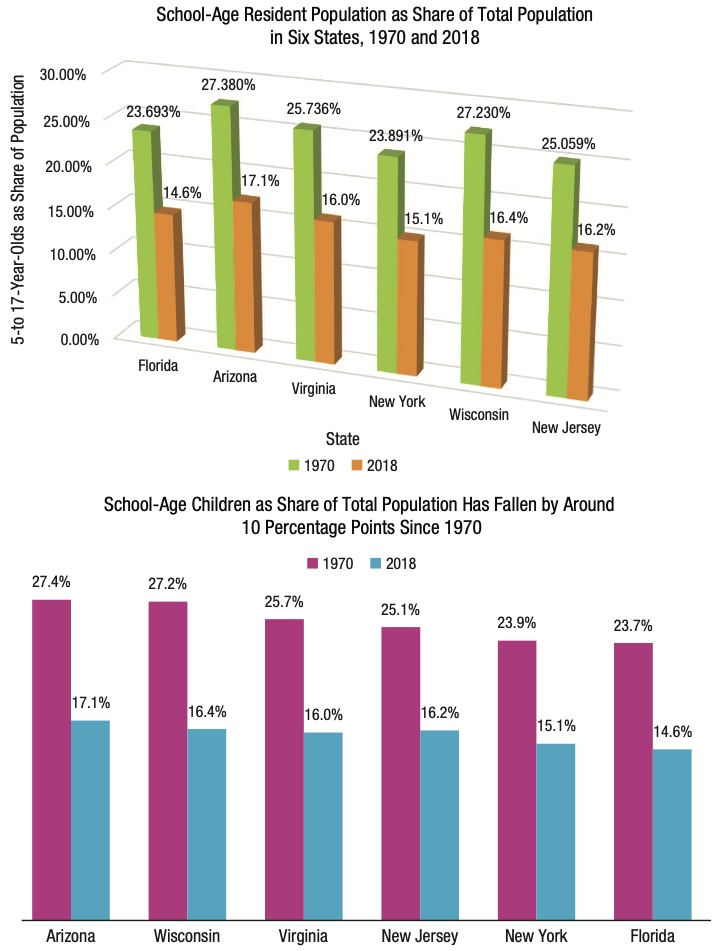
\includegraphics[width=.8\linewidth]{figs/100-barchart-redesign.jpg}
\caption{Primer izboljšanja stolpčnega diagrama. Zgornji graf uporablja tridimenzionalni prikaz, močne mreže in nepregledne oznake, spodnji pa enostavnejšo postavitev, neposredno označevanje podatkov in bolj pregledno uporabo barv. Povzeto po Schwabish (2021). Odstranitev nepotrebnih grafičnih elementov bistveno izboljša preglednost in usmeri pozornost na podatke namesto na dekoracijo. Takšni odvečni elementi so pogosto označeni z izrazom \emph{chartjunk}, ki opisuje grafične dodatke brez analitične vrednosti.
\protect\label{fig:design-bar-redesign}}
\end{figure}
%
Graf naj vsebuje le elemente, ki prispevajo k razumevanju podatkov. Nepotrebni dekorativni učinki, tridimenzionalni prikazi, ogromna omrežja ali pretirano število oznak pogosto zmanjšajo preglednost in otežijo interpretacijo. Glavno sporočilo vizualizacije mora biti razvidno takoj. Opazovalec ne bi smel ugibati, kaj graf prikazuje ali kateri podatki so pomembni. Ključne informacije morajo biti vizualno poudarjene, manj pomembni elementi pa umaknjeni v ozadje.

\vspace{1em}
\noindent {\bf Vizualna hierarhija in usmerjanje pozornosti.}
Dobra vizualizacija mora opazovalca usmerjati k najpomembnejšim informacijam. Vizualna hierarhija določa, katere elemente zaznamo najprej in katere kasneje. To dosežemo z uporabo kontrasta, velikosti, debeline črt, položaja ali barve. Pogosto želimo poudariti le manjši del podatkov, medtem ko preostale informacije ostanejo v ozadju. Zato številni sodobni grafi uporabljajo nevtralne sive tone za večino elementov, ključne podatke pa poudarijo z izrazitejšo barvo. Tak pristop zmanjša vizualni šum in omogoči hitrejše razumevanje bistvenih informacij. Vizualna hierarhija je posebej pomembna pri kompleksnih grafih, kjer bi enakovredno poudarjanje vseh elementov povzročilo nepreglednost in povečalo kognitivno obremenitev opazovalca.
%
\begin{figure}[htb]
\centering
% Figure 6 iz Schwabish (2021): uporaba dot plota in vizualne hierarhije
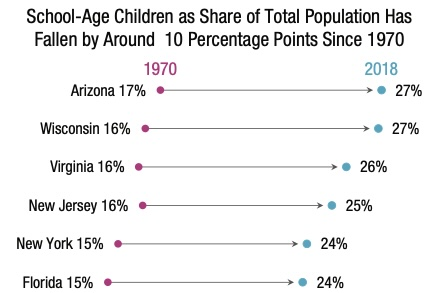
\includegraphics[width=.6\linewidth]{figs/100-design-dotplot.jpg}
\caption{Točkovni prikaz uporablja nevtralne elemente in poudarjene oznake za usmerjanje pozornosti opazovalca na ključne razlike med podatki. Neposredno označevanje podatkov zmanjšuje potrebo po ločenih legendah in izboljša preglednost vizualizacije. Povzeto po Schwabish (2021).
\protect\label{fig:design-dotplot-highlight}}
\end{figure}
%

\vspace{1em}
\noindent {\bf Doslednost in zmanjševanje kognitivne obremenitve.}
Vizualizacije morajo uporabljati dosledne grafične konvencije. Enake barve naj predstavljajo iste kategorije, osi naj uporabljajo enake merske enote, tipografija in oznake pa naj bodo poenotene skozi celotno predstavitev. 

Nedoslednosti povečajo kognitivno obremenitev, saj mora opazovalec ponovno interpretirati pomen posameznih elementov. Vizualizacija mora biti zasnovana tako, da opazovalec čim manj časa porabi za razumevanje same strukture grafa in čim več za interpretacijo podatkov. Kognitivno obremenitev zmanjšujemo tudi z neposrednim označevanjem podatkov namesto ločenih legend, z uporabo kratkih in informativnih naslovov ter z logično razporeditvijo elementov. Posebej učinkovite so vizualizacije, kjer so besedilo, oznake in grafični elementi tesno povezani.

%
\begin{figure}[htb]
\centering
% kombinacija Figure 5 in Figure 6 iz Schwabish (2021): bar chart vs dot plot
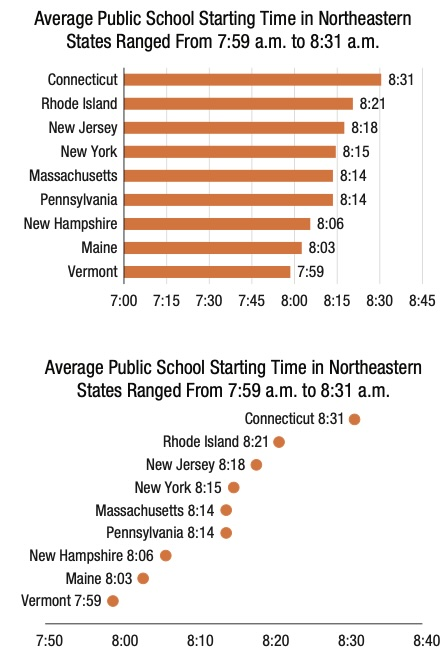
\includegraphics[width=.3\linewidth]{figs/100-design-bar-dotplot.jpg}
\caption{Primerjava stolpčnega diagrama in točkovnega prikaza. Točkovni prikaz uporablja manj vizualnega prostora in omogoča hitrejše primerjanje vrednosti ter sprememb med kategorijami. Povzeto po Schwabish (2021).
\protect\label{fig:design-dotplot}}
\end{figure}
%

\vspace{1em}
\noindent {\bf Barve in dostopnost.}
Barva je eden najmočnejših vizualnih elementov, vendar jo moramo uporabljati previdno. Primerna je predvsem za razlikovanje kategorij, poudarjanje pomembnih podatkov in prikaz intenzitete vrednosti. Pomemben delež populacije ima različne oblike motenj barvnega zaznavanja, najpogosteje težave pri razlikovanju rdeče in zelene barve. Vizualizacije morajo zato ostati razumljive tudi uporabnikom z barvno slepoto ter pri sivinskem prikazu. Zato se pogosto izogibamo problematičnim kombinacijam ter uporabljamo perceptualno primerne barvne lestvice.

\vspace{1em}
\noindent {\bf Oblikovne odločitve vplivajo na interpretacijo.}
Na interpretacijo podatkov močno vpliva tudi način njihove vizualne predstavitve. Že majhne oblikovne odločitve lahko močno vplivajo na interpretacijo in ustvarijo napačen vtis o trendih ali razlikah med podatki. Posebej problematične so neustrezne osi, pretirano poudarjeni elementi ali neprimerna uporaba linij in površin. Takšne odločitve lahko povzročijo, da opazovalec zazna trend ali povezavo, ki v podatkih dejansko ne obstaja.
%
\begin{figure}[htb]
\centering
% Figure 3 iz Schwabish (2021): primer zavajajoče uporabe obrnjene osi
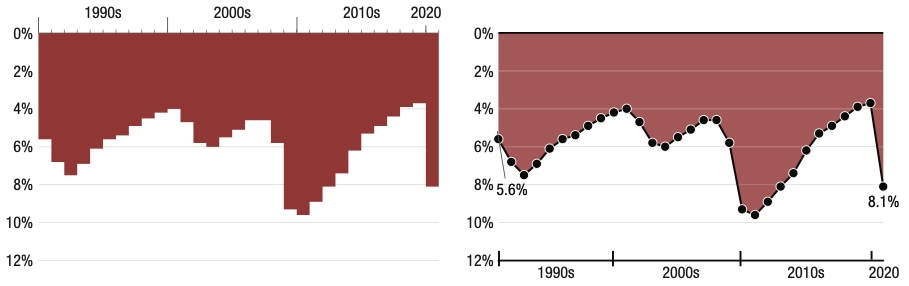
\includegraphics[width=.95\linewidth]{figs/100-design-axis-example.jpg}
\caption{Dve vizualizaciji istih podatkov z obrnjeno navpično osjo. Leva različica uporablja stolpce in pravilno poudarja dolžino kot nosilko informacije, desna pa zaradi linije in položaja točk ustvarja zavajajoč vtis trenda. Povzeto po Schwabish (2021).
\protect\label{fig:design-axis-example}}
\end{figure}
%


Učinkovita vizualizacija zato zahteva več kot zgolj tehnično znanje izdelave grafov. Zahteva razumevanje človekove percepcije, načel grafične komunikacije ter prilagoditev ciljnemu občinstvu. Dobra vizualizacija opazovalcu olajša razumevanje podatkov in odnosov med njimi.

%%%%

\section{Zavajajoče vizualizacije}

Vizualizacije podatkov imajo velik vpliv na razumevanje informacij, zato lahko že majhne oblikovne odločitve bistveno spremenijo interpretacijo podatkov.
%
\marginnote{Nekateri primeri v tem razdelku so povzeti po članku \emph{The Science of Visual Data Communication: What Works} (Franconeri idr., 2021), ki vključuje tudi primere napak in zavajajoče načine prikaza podatkov.}
%
Grafi pogosto delujejo objektivno in znanstveno, vendar lahko z neustreznim oblikovanjem ustvarijo zavajajoč vtis o velikosti razlik, trendih ali povezavah med spremenljivkami. Zaradi tega je etično oblikovanje vizualizacij pomemben del odgovorne komunikacije podatkov.

\vspace{1em}
\noindent {\bf Prirezane osi in popačene skale.}
Eden najpogostejših načinov zavajanja je uporaba prirezanih osi. Če navpična os ne začne pri nič, lahko že majhne razlike med vrednostmi delujejo bistveno večje, kot so v resnici. Takšne manipulacije pogosto pretirano poudarijo trende ali razlike med skupinami. Podoben učinek imajo popačene skale, kjer razmiki med vrednostmi niso linearni ali pa so vizualno predstavljeni nesorazmerno glede na dejanske podatke. Opazovalec običajno zazna predvsem vizualno velikost razlik in manj pogosto natančno preverja numerične vrednosti na osi. Takšni prijemi so pogosti v medijih, politiki in poslovnih predstavitvah, kjer želimo določene razlike poudariti bolj, kot to upravičujejo podatki.
%
\begin{figure}[t]
\centering
% Figure 3 iz Franconeri et al. (2021): zavajajoče osi in raztegovanje skale
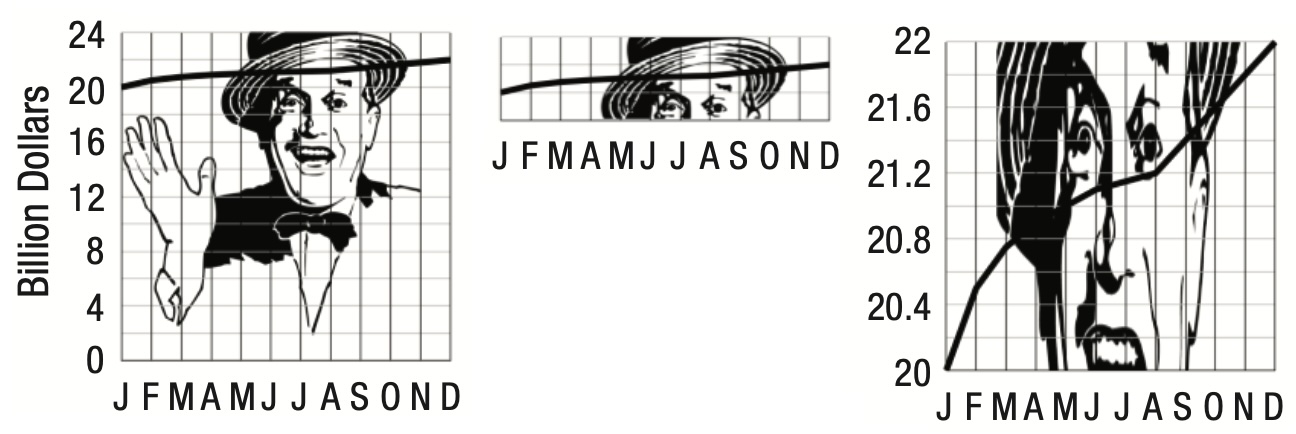
\includegraphics[width=.95\linewidth]{figs/100-err-truncated-axis.jpg}
\caption{Primer vpliva prirezanih osi in raztegnjenih skal na interpretacijo podatkov. Enaki podatki lahko zaradi drugačne izbire osi ustvarijo bistveno drugačen vtis o velikosti razlik ali trendov. Povzeto po Franconeri in sod. (2021).
\protect\label{fig:ethics-truncated-axis}}
\end{figure}
%

\vspace{1em}
\noindent {\bf Zavajajoče barvne lestvice.}
Barva močno vpliva na zaznavanje intenzitete podatkov. Neprimerne barvne lestvice lahko ustvarijo umetne meje med vrednostmi ali poudarijo razlike, ki v podatkih niso pomembne. Posebej problematične so lestvice z močnimi prehodi med različnimi barvnimi kategorijami, na primer med modro, zeleno in rdečo. Človek zazna prehod med barvnimi kategorijami kot večjo razliko, kot dejansko obstaja v podatkih. Zaradi tega lahko kontinuirani podatki delujejo bolj diskretno ali dramatično. Pri oblikovanju vizualizacij zato uporabljamo perceptualno enakomerne barvne lestvice, kjer sprememba barve čim bolj ustreza dejanski spremembi podatkovnih vrednosti.

\vspace{1em}
\noindent {\bf Prekrivanje podatkov in izbira prikazanih primerov.}
Pri velikih množicah podatkov lahko pride do prekrivanja točk (\emph{overplotting}), kjer posamezne vrednosti zakrijejo druge. Posledično lahko pomembni vzorci ostanejo skriti ali pa vizualizacija daje napačen vtis gostote podatkov. Zavajajoč učinek lahko povzroči tudi selektivna izbira podatkov (angl. \emph{cherry-picking}), kjer avtor prikaže le tiste podatke, ki podpirajo želeni zaključek. Vizualizacija lahko tako deluje prepričljivo, čeprav ne predstavlja celotne slike. Zato morajo vizualizacije jasno prikazati obseg podatkov, uporabljene filtre in morebitne omejitve pri izbiri vzorca.

\vspace{1em}
\noindent {\bf Korelacija ni vzročnost.}
Vizualizacije pogosto učinkovito pokažejo povezave med spremenljivkami, vendar povezava sama po sebi še ne pomeni vzročne zveze. Dve spremenljivki sta lahko močno povezani, čeprav med njima ni neposrednega vpliva. Razsevni in linijski diagrami lahko hitro ustvarijo vtis vzročne povezave, posebej kadar sta podatka prikazana skupaj skozi čas. Opazovalci pogosto intuitivno sklepajo, da ena spremenljivka povzroča drugo, čeprav je povezava lahko posledica tretjega dejavnika ali naključja. Slika~\ref{fig:ethics-patterns} prikazuje, kako hitro opazimo vzorce in strukture v podatkih, tudi kadar ti niso nujno analitično pomembni. Pri interpretaciji vizualizacij moramo zato ločiti med opisom podatkov in dejanskimi vzročnimi razlagami.
%
\begin{marginfigure}
\centering
% Figure 7 iz Franconeri et al. (2021): omejitve vizualnega primerjanja in zaznavanja vzorcev
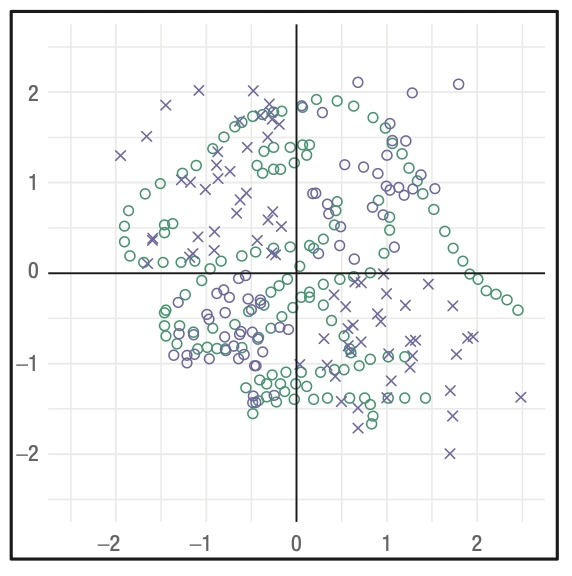
\includegraphics[width=.9\linewidth]{figs/100-err-patterns.jpg}
\caption{Človekov vizualni sistem hitro zaznava vzorce in povezave med podatki, vendar lahko to vodi tudi do napačnega sklepanja o odnosih med spremenljivkami. Povzeto po Franconeri idr. (2021).
\protect\label{fig:ethics-patterns}}
\end{marginfigure}
%

\vspace{1em}
\noindent {\bf Prikazovanje negotovosti.}
Podatki pogosto vsebujejo negotovost, ki jo moramo ustrezno prikazati. Če negotovosti ne pokažemo, lahko vizualizacija daje lažen vtis natančnosti in gotovosti. Negotovost običajno prikazujemo z intervali zaupanja, območji verjetnosti, razponi napak ali več možnimi scenariji. Posebej pomembno je to pri vremenskih napovedih, epidemioloških modelih, ekonomskih napovedih in znanstvenih rezultatih. Vizualizacija mora zato jasno pokazati:
\begin{itemize}
\item katere podatke prikazujemo,
\item kakšna je stopnja negotovosti,
\item katere omejitve imajo podatki,
\item in katerih zaključkov iz vizualizacije ne moremo zanesljivo sklepati.
\end{itemize}

%%%%%%

\section{Primeri izbire in izboljšanja vizualnih predstavitev}

Iste podatke lahko prikažemo na več načinov, pri čemer vsak način poudari nekoliko drug vidik: prostorski vzorec, primerjavo med enotami, povezavo med spremenljivkami, natančne vrednosti ali bolj intuitivno razumevanje časovnih podatkov. V nadaljevanju si ogledamo nekaj primerov iz članka Schwabisha (2021) v reviji {\em Psychological Science in the Public Interest}, ki pokažejo, kako lahko že razmeroma preproste spremembe izboljšajo razumljivost in uporabnost vizualizacije. Avtor pri tem uporablja podatke o začetku pouka v javnih šolah v ZDA ter pokaže, da lahko tudi z običajnimi orodji pripravimo precej različne, a učinkovite predstavitve podatkov.

\vspace{1em}
\noindent {\bf Prostorski podatki.}
Pri prostorskih podatkih pogosto najprej pomislimo na običajen zemljevid, vendar ta ni vedno najboljša izbira. Klasični koropletni zemljevid dobro ohranja geografsko obliko držav in zato hitro razkrije prostorske vzorce, na primer da se pouk v južnih zveznih državah začne nekoliko prej. Po drugi strani velikost geografskih območij vpliva na zaznano pomembnost podatkov: velike države na zemljevidu zavzamejo več prostora, čeprav nimajo nujno večje analitične teže. Mrežni zemljevid s ploščicami ta problem zmanjša, saj vsaki državi nameni enako velik prostor, hkrati pa omogoča dodajanje oznak ali majhnih grafičnih elementov znotraj vsake celice (slika~\ref{fig:schwabish-maps}). Tak prikaz žrtvuje nekaj geografske natančnosti, vendar lahko izboljša primerljivost in poveča uporabnost prikaza za bralca.

\begin{figure}[t]
\centering
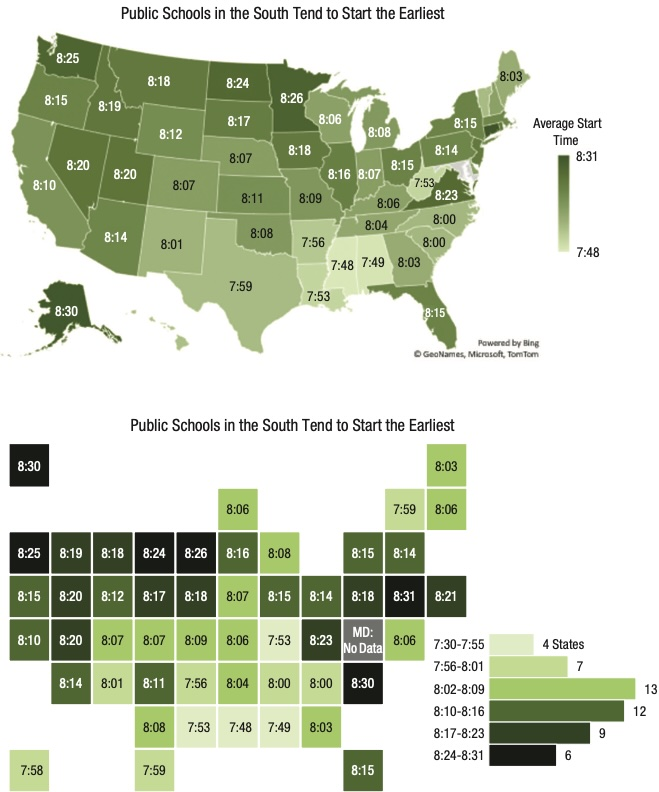
\includegraphics[width=.95\linewidth]{figs/100-schwa-maps.jpg}
\caption{Dva načina prikaza prostorskih podatkov o povprečnem začetku pouka v javnih šolah v ZDA: običajni koropletni zemljevid in mrežni zemljevid s ploščicami. Prvi bolje ohranja geografsko obliko, drugi pa vsaki državi nameni enak prostor in tako olajša primerjavo med državami.
\protect\label{fig:schwabish-maps}}
\end{figure}

\vspace{1em}
\noindent {\bf Stolpci ali točke.}
Stolpčni diagram je ena najbolj znanih in razumljivih vizualizacij za primerjanje vrednosti med skupinami. Njegova prednost je, da dolžine stolpcev primerjamo razmeroma natančno, še posebej, kadar imajo skupno izhodišče. Toda stolpčni diagrami lahko postanejo vizualno težki, posebej pri večjem številu kategorij ali daljših oznakah. Točkovni diagram za iste podatke pogosto uporablja manj grafičnega prostora in pusti več prostora za oznake, komentarje ali neposredno označevanje vrednosti (slika~\ref{fig:schwabish-bars-dots}). Primer zato ne kaže, da je stolpčni diagram napačen, ampak da lahko preprostejša in lažja grafična oblika bolj berljiva, kadar nas zanima predvsem vrstni red in primerjava posameznih vrednosti.

\begin{figure}[t]
\centering
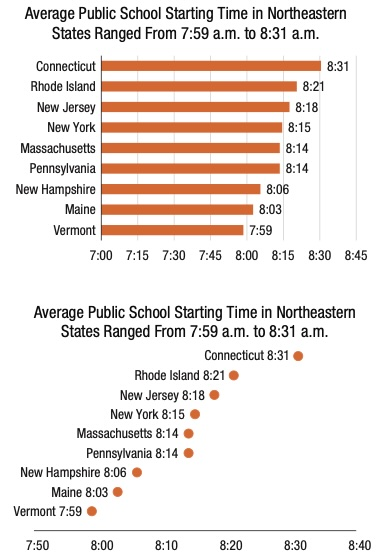
\includegraphics[width=.75\linewidth]{figs/100-schwa-bars-dots.jpg}
\caption{Primerjava stolpčnega diagrama in točkovnega prikaza za iste podatke. Stolpci omogočajo neposredno primerjavo dolžin, točkovni prikaz pa zmanjša vizualno težo grafa in omogoči preglednejše označevanje vrednosti.
\protect\label{fig:schwabish-bars-dots}}
\end{figure}

\vspace{1em}
\noindent {\bf Razsevni diagram kot prostor za razlago.}
Razsevni diagram je osnovni prikaz za raziskovanje povezave med dvema numeričnima spremenljivkama. Vendar dober razsevni diagram ni le oblak točk. Z dodatnimi oznakami, povprečnimi črtami, pojasnili osi in označenimi osamelci lahko bralcu pomagamo razumeti, kaj naj v grafu opazi. Pri podatkih o začetku pouka in deležu šoloobveznih otrok v populaciji lahko vodoravne in navpične referenčne črte razdelijo prostor grafa na območja nad in pod povprečjem, oznake izbranih držav pa usmerijo pozornost na primere, ki posebej odstopajo (slika~\ref{fig:schwabish-scatter}). Pri takem prikazu je pomembno ravnotežje: preveč oznak graf obremeni, premišljene oznake pa lahko bistveno izboljšajo interpretacijo.

\begin{figure}[t]
\centering
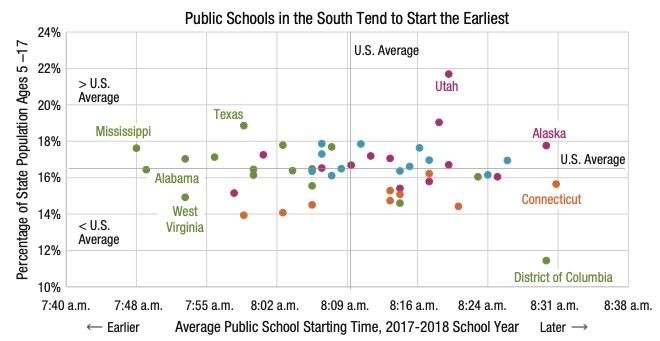
\includegraphics[width=.95\linewidth]{figs/100-schwa-scatter.jpg}
\caption{Razsevni diagram povezave med povprečnim začetkom pouka in deležem prebivalstva v starosti od 5 do 17 let. Referenčne črte, oznake osi in izbrane oznake držav pomagajo bralcu razumeti strukturo podatkov ter prepoznati osamelce.
\protect\label{fig:schwabish-scatter}}
\end{figure}

\vspace{1em}
\noindent {\bf Tudi tabela je vizualizacija.}
Tabele pogosto razumemo kot nasprotje grafov, vendar so tudi tabele oblika vizualne predstavitve podatkov. Slabo oblikovana tabela oteži primerjanje vrednosti: glave stolpcev niso jasno ločene, besedilo in številke niso ustrezno poravnani, število decimalnih mest je nedosledno, enote pa so zapisane neenotno. Z razmeroma majhnimi popravki lahko tabela postane bistveno preglednejša: glave stolpcev so jasno ločene, besedilo je levo poravnano, številke desno poravnane, natančnost zapisa je poenotena, dodani majhni stolpci v zadnjem stolpcu pa pomagajo hitro zaznati vzorec (slika~\ref{fig:schwabish-table}). Tak primer je posebej pomemben za poročila in znanstvena besedila, kjer tabele pogosto nosijo veliko informacij.

\begin{figure}[t]
\centering
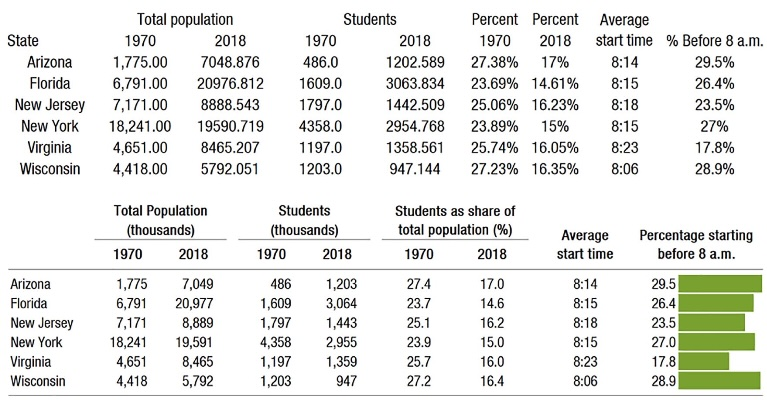
\includegraphics[width=.95\linewidth]{figs/100-schwa-table.jpg}
\caption{Primer izboljšanja tabele. Preglednejša različica uporablja jasnejšo hierarhijo glave, ustrezno poravnavo besedila in številk, enotno število decimalnih mest ter majhne stolpčne prikaze za hitrejše zaznavanje vzorcev. Povzeto po Schwabish (2021), Figure~10.
\protect\label{fig:schwabish-table}}
\end{figure}

\vspace{1em}
\noindent {\bf Vizualizacija, ki izhaja iz pomena podatkov.}
Kadar podatki opisujejo čas dneva, lahko vizualizacija izkoristi obliko, ki je bralcu že znana iz vsakdanjega življenja. Namesto zemljevida, stolpčnega grafa ali tabele lahko začetke pouka razporedimo po številčnici ure, kjer položaj oznake neposredno ustreza času začetka (slika~\ref{fig:schwabish-clock}). Tak prikaz ni nujno najbolj standarden, vendar je dobro usklajen s pomenom podatkov: bralec takoj razume, da gre za čas, in lahko poišče posamezno državo na znani krožni strukturi. Primer kaže, da je lahko nekoliko bolj igriva ali nestandardna vizualizacija še vedno analitično smiselna, če podpira razumevanje podatkov in ne zakriva njihovega pomena.

\begin{figure}[t]
\centering
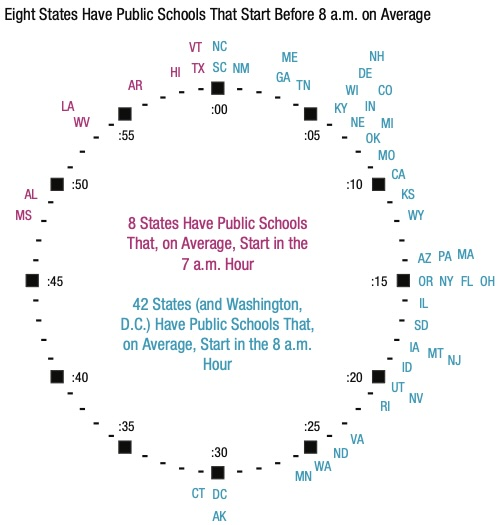
\includegraphics[width=.7\linewidth]{figs/100-schwa-clock.jpg}
\caption{Alternativni prikaz časovnih podatkov s številčnico ure. Oznake držav so razporejene glede na povprečni čas začetka pouka, barva pa dodatno loči države, kjer se pouk v povprečju začne pred osmo uro.
\protect\label{fig:schwabish-clock}}
\end{figure}

Skupno sporočilo teh primerov je, da učinkovita vizualizacija nastane iz povezave med podatki, nalogo in občinstvom. Ni dovolj, da izberemo prvi graf, ki ga ponudi programsko orodje. Premisliti moramo, kaj želimo poudariti, katere primerjave naj bralec opravi, koliko razlage potrebuje in kateri prikaz bo podatke predstavil najbolj jasno. Včasih je to običajen stolpčni diagram, drugič zemljevid, tabela, točkovni prikaz ali celo ura.

%%%%%%
\section{Vizualna analitika in interaktivnost}

Sodobna vizualizacija podatkov ni več omejena le na statične slike v tiskanih medijih (članki, poročila) ali na drsnicah. Vedno pomembnejšo vlogo imajo interaktivne vizualizacije, pri katerih lahko uporabnik podatke raziskuje, spreminja pogled na podatke in se osredotoča na zanimive podmnožice podatkov. Tak pristop uporabljajo tehnike \emph{vizualne analitike}, ki združujejo vizualizacijo, interakcijo in analitično raziskovanje podatkov.

Ko uporablja vizualne vmesnike, uporabnik ni le pasivni opazovalec grafične predstavitve, ampak lahko aktivno spreminja prikaz podatkov in, kolikor mnu vmesnik dopušča, preiskuje in raziskuje podatke. Najpogostejše interakcije, ki jih taki sistemi implementirajo, vključujejo:
\begin{itemize}
    \item \textbf{filtriranje}, kjer izberemo le del podatkov,
    \item \textbf{brushing}, kjer označimo podmnožico podatkov v enem prikazu,
    \item \textbf{povečevanje in premikanje} (\emph{zooming} in \emph{panning}), kjer se lahko osredotočimo na del podatkov,
    \item \textbf{izbiro elementov} (\emph{selection}), kjer v eni vizualizaciji izberemo elemente, ki jih potem navadno prikažemo na dodatni vizualizaciji,
    \item \textbf{podrobnosti na zahtevo} (\emph{details on demand}), kjer se dodatne informacije prikažejo ob kliku miške ali ko stojimo z miško na določenem elementu, za katerega nas zanimjo dodatne podrobnosti, in
    \item \textbf{barvanje in označevanje skupin}, kjer na grafični način uporabnik razdeli podatke v njemu zanimive skupine, za katere je potem seveda potrebno prikazati razlike z dodatnimi prikazi ali v dodatnih vizualizacijah.
\end{itemize}

V preiskovalne namene so posebej uporabne povezane vizualizacije (\emph{linked visualizations}). Pri takem pristopu izbira podatkov v enem grafu (avtomatičo in hipno) vpliva tudi na druge prikaze. Če na primer v razsevnem diagramu označimo določeno skupino podatkov, se isti podatki istočasno označijo tudi v histogramu ali tabeli. Tak način omogoča učinkovito raziskovanje večdimenzionalnih podatkov in hitro odkrivanje povezav med atributi.

Interaktivne vizualizacije pogosto združujemo v nadzorne plošče oziroma \emph{dashboards}. Ti prikazi vsebujejo več med seboj povezanih grafov, filtrov in tabel, ki uporabniku omogočajo pregled nad podatki in interaktivno analizo. Podoben pristop uporabljajo tudi sistemi za vizualno podatkovno analitiko, kot je ljubljanski Orange Data Mining, kjer uporabnik gradi analitični potek dela (\emph{workflow}) s povezovanjem posameznih komponent za uvoz podatkov, analizo, modeliranje in vizualizacijo in na ta način določi način obdelave podatkov ter med sabo poveže vizualizacije.

Podporo za interaktivno vizualizacijo danes ponujajo številna programska orodja. Tableau je eno najbolj razširjenih okolij za pripravo interaktivnih nadzornih plošč in raziskovalno analizo podatkov, saj omogoča hitro povezovanje grafov, filtrov in interaktivnih pogledov brez programiranja. Podobno vlogo ima Microsoft Power BI, ki je močno povezan z ekosistemom podatkovnih storitev podjetja Microsoft in se pogosto uporablja za poslovno analitiko ter spremljanje podatkov v realnem času. Orodja, kot je Orange Data Mining, KNIME in RapidMiner, pa so bolj usmerjena v raziskovalno analizo in strojno učenje, kjer uporabnik z vizualnim povezovanjem komponent gradi celoten analitični potek dela. Skupna značilnost teh sistemov je podpora interaktivnosti, povezanim vizualizacijam ter postopnemu raziskovanju podatkov.

Poseben izziv predstavljajo podatki v realnem času oziroma pretočni podatki (\emph{streaming data}). Pri takih podatkih se vizualizacija sproti posodablja, ko prihajajo novi podatki. Takšne prikaze srečamo pri spremljanju omrežnega prometa, finančnih trgov, senzorjev ali družbenih omrežij. Poleg samega prikaza podatkov je pri takih sistemih pomembna tudi hitrost osveževanja, poudarjanje pomembnih sprememb ter preprečevanje preobremenitve uporabnika z informacijami.

Interaktivnost zato ni le estetski dodatek, ampak pomembno orodje za raziskovanje podatkov. Dobro zasnovane interaktivne vizualizacije uporabniku omogočajo, da sam raziskuje podatke, postavlja vprašanja in postopoma gradi razumevanje analiziranega problema.


\section{Pripovedovanje zgodb s podatki}

Vizualizacija podatkov je predvsem način komunikacije o spoznanjih, ki smo jih na osnovi podatkov pridobili. Pri pripravi vizualizacije zato običajno pričnemo z vprašanjem, kaj želimo sporočiti. Isti podatki lahko podprejo različne zgodbe: lahko poudarimo trend, primerjavo, izjemen primer, negotovost ali spremembo skozi čas. Naloga avtorja vizualizacije je, da izbere prikaze ali redosled prikazov, ki podprejo glavno sporočilo, ter usmeri pozornost bralca na pomembne dele podatkov in vzorce. Pri tem imajo pomembno vlogo barva, kontrast, velikost elementov, označevanje in komentarji (\emph{annotation}), s katerimi lahko poudarimo ključne informacije in zmanjšamo vpliv manj pomembnih podrobnosti.

Učinkovita vizualizacija podatkov zato pogosto deluje kot pripoved (\emph{storytelling with data}). Bralca vodi skozi podatke, postopoma razkriva pomembne vzorce in pomaga pri interpretaciji rezultatov. Tak pristop je posebej značilen za novinarske in spletne interaktivne vizualizacije, kjer uporabnik podatke raziskuje korak za korakom. Pri tem moramo vedno upoštevati tudi občinstvo: vizualizacije za strokovnjake lahko vsebujejo več podrobnosti in kompleksnejše prikaze, medtem ko morajo biti vizualizacije za širšo javnost bolj neposredne in hitro razumljive. Dobra vizualizacija zato ne prikazuje le podatkov, ampak pomaga oblikovati razumevanje problema.


\section{Programska orodja za gradnjo vizualizacij}

Vizualizacije podatkov danes pogosto ne nastajajo več kot ročno narisane slike,
temveč kot rezultat programskega opisa podatkov, njihovih preslikav v vizualne
elemente in pravil interakcije. Tak pristop je posebej pomemben v podatkovni
znanosti, kjer želimo grafe graditi ponovljivo, jih prilagajati novim podatkom
in jih vključevati v poročila, spletne strani ali interaktivna analitična okolja.

Najpreprostejši primer takega pristopa v Pythonu je uporaba knjižnice
\texttt{matplotlib}. Ta omogoča natančen nadzor nad posameznimi elementi grafa
in je osnova številnih drugih vizualizacijskih knjižnic.

\vspace*{3mm}
\begin{lstlisting}
import matplotlib.pyplot as plt

x = [1, 2, 3, 4, 5]
y = [2.1, 2.8, 3.6, 3.9, 5.1]

plt.figure()
plt.scatter(x, y)
plt.xlabel("stevilo ur ucenja")
plt.ylabel("rezultat")
plt.savefig("scatter.pdf", bbox_inches="tight")
\end{lstlisting}

Koda zgradi enostaven razsevni diagram, kjer vsaka točka predstavlja en primer.
Tak prikaz je tipičen za raziskovanje povezave med dvema numeričnima
spremenljivkama. Knjižnica \texttt{matplotlib} je nekoliko bolj nizkonivojska,
zato moramo sami določiti osi, oznake, legende in druge grafične elemente.

Za statistične prikaze pogosto uporabimo knjižnico \texttt{seaborn}, ki gradi na
\texttt{matplotlibu}, vendar ponuja višjenivojske funkcije za pogoste tipe grafov.

\vspace*{3mm}
\begin{lstlisting}
import seaborn as sns
import pandas as pd

d = pd.DataFrame({
    "skupina": ["A", "A", "A", "B", "B", "B"],
    "vrednost": [4.1, 5.0, 4.7, 6.2, 5.8, 6.5],
})

sns.boxplot(data=d, x="skupina", y="vrednost")
plt.savefig("boxplot.pdf", bbox_inches="tight")
\end{lstlisting}

V tem primeru zgradimo škatlo z brki za primerjavo porazdelitev med dvema
skupinama. Prednost knjižnice \texttt{seaborn} je, da neposredno razume podatkovne
tabele, kakršne uporabljamo v knjižnici \texttt{pandas}, in zato omogoča hitro
gradnjo raziskovalnih grafov.

Drugačen pristop uporablja knjižnica \texttt{Altair}. Ta temelji na jeziku
\texttt{Vega-Lite}, kjer vizualizacijo opišemo deklarativno: določimo podatke,
vrsto grafa in preslikave stolpcev v vizualne elemente, knjižnica pa iz tega
sestavi končno vizualizacijo.

\vspace*{3mm}
\begin{lstlisting}
import altair as alt
import pandas as pd

d = pd.DataFrame({
    "ure": [1, 2, 3, 4, 5],
    "rezultat": [2.1, 2.8, 3.6, 3.9, 5.1],
})

chart = alt.Chart(d).mark_point().encode(
    x="ure",
    y="rezultat",
)

chart.save("altair-scatter.html")
\end{lstlisting}

Pri tem programu ne določamo neposredno, kako naj se izriše vsaka točka.
Namesto tega povemo, da naj bodo vrednosti stolpca \texttt{ure} prikazane na osi
\(x\), vrednosti stolpca \texttt{rezultat} pa na osi \(y\). Tak deklarativni
pristop je bližje formalnim jezikom za opis vizualizacij.

Med najpomembnejšimi formalnimi jeziki za opise vizualizacij danes štejemo \texttt{Vega} in \texttt{Vega-Lite}.
Oba uporabljata zapise v obliki JSON. \texttt{Vega-Lite} je višjenivojski in
primeren za običajne statistične grafe, \texttt{Vega} pa omogoča podrobnejši
nadzor nad transformacijami podatkov, interakcijami in grafičnimi elementi.
Knjižnica \texttt{Altair} je pravzaprav Pythonov vmesnik za gradnjo
\texttt{Vega-Lite} specifikacij.

Za bolj proste in unikatne spletne vizualizacije se pogosto uporablja
\texttt{D3.js}. Ta ni deklarativni jezik v istem smislu kot \texttt{Vega}, temveč
JavaScript knjižnica, ki podatke poveže z elementi spletne strani, na primer z
elementi SVG. D3 omogoča zelo veliko prilagodljivost, vendar zahteva tudi več
programiranja.

Interaktivne vizualizacije lahko v Pythonu gradimo tudi s knjižnico
\texttt{plotly}. Njeni grafi so spletni objekti, zato jih lahko odpremo v
brskalniku, vključimo v spletno stran ali uporabimo v interaktivnih zvezkih.

\vspace*{3mm}
\begin{lstlisting}
import plotly.express as px
import pandas as pd

d = pd.DataFrame({
    "ure": [1, 2, 3, 4, 5],
    "rezultat": [2.1, 2.8, 3.6, 3.9, 5.1],
    "skupina": ["A", "A", "B", "B", "B"],
})

fig = px.scatter(
    d, x="ure", y="rezultat", color="skupina",
    hover_data=["skupina"]
)

fig.write_html("plotly-scatter.html")
\end{lstlisting}

Interaktivne vizualizacije lahko gradimo tudi deklarativno, kjer ne opisujemo
posameznih grafičnih elementov, temveč povezave med podatki, vizualnimi
atributi in interakcijami. Tak pristop posebej dobro podpira knjižnica
\texttt{Altair}, ki temelji na jeziku \texttt{Vega-Lite}. Naslednji primer prikazuje dva povezana grafa. V levem razsevnem diagramu lahko uporabnik z miško izbere skupino točk, histogram na desni pa nato prikaže porazdelitev samo za izbrane primere.
%
\vspace*{3mm}
\begin{lstlisting}
import altair as alt
from vega_datasets import data

d = data.cars()

brush = alt.selection_interval()

scatter = alt.Chart(d).mark_point(size=60).encode(
    x="Horsepower:Q",
    y="Miles_per_Gallon:Q",
    color="Origin:N"
).add_params(brush)

hist = alt.Chart(d).mark_bar().encode(
    x=alt.X("Miles_per_Gallon:Q", bin=True),
    y="count()",
    color="Origin:N"
).transform_filter(brush)

chart = scatter | hist
chart.save("linked-view.html")
\end{lstlisting}
% 
Zgoraj smo sicer vizualizacijo shranili v datoteko HTML, a še bolj primerno bi bilo kodo uporabiti v interaktivnih okoljih kot je Marimo.

\section{Vizualizacija podatkov in umetna inteligenca}

Čeprav smo se v vseh poglavjih do tega ukvarjali s strojnim učenjem in torej podlagami za umetno inteligenco, o povezavi te z vizualizacijami nismo napisali ničesar. Čas je, da v tej smeri zaključimo. Namreč, vizualizacija podatkov in umetna inteligenca skupaj odpirata izjemno širok prostor novih pristopov in raziskovalnih vprašanj. Umetna inteligenca lahko pomaga pri samodejnem oblikovanju vizualizacij, izbiri ustreznih prikazov ter prilagajanju predstavitev različnim uporabnikom in kontekstom. Vizualizacije vse bolj postajajo del pogovornih vmesnikov, kjer modeli ne odgovarjajo več le z besedilom, temveč tudi z dinamičnimi grafičnimi prikazi, ki podpirajo razlago, raziskovanje podatkov in skupno razmišljanje. Umetna inteligenca bo imela izjemno pomembno vlogo pri razlagi podatkov in razložljivih vizualizacijah, torej vizualizacijah, kjer bomo s prijemi umetne inteligence v vizualizacije vključevali vsebine, ki te dodatno razložijo, ali pa sploh poiskali vizualizacije, ki so razložljive in odgovorijo na uporabnikovo vprašanje.

Pomembno področje postaja tudi oblikovanje zgodb z uporabo podatkov, kjer se prepletajo analiza, pisna zgodba in vizualna komunikacija. Ob tem se odpirajo še številne druge možnosti: interaktivna razlaga kompleksnih modelov, generiranje vizualnih analitičnih povzetkov, sodelovanje med človekom in modelom pri raziskovanju podatkov ter razvoj novih načinov vizualnega razmišljanja, kjer umetna inteligenca ne nastopa le kot orodje za analizo, temveč kot sogovornik in soustvarjalec interpretacij.